% {{{1 PRELUDE
\documentclass{beamer}

% Packages
\usepackage[english]{babel}
\usepackage[utf8]{inputenc}
\usepackage[T1]{fontenc}
\usepackage{amsmath,amssymb}
\usepackage{bbm}

% Custom commands
\newcommand{\R}{\mathbb{R}}
\newcommand{\indicator}[1]{\mathbbm{1}_{#1}}
\newcommand{\meanv}[1]{\vec{H}_{#1}}

\usetheme{Frankfurt}

% Add slide numbering
\useoutertheme{infolines}
\setbeamertemplate{headline}{} % removes the headline that infolines inserts

% Remove navigation symbols
\beamertemplatenavigationsymbolsempty

\AtBeginSection[]
{
    \begin{frame}
        \frametitle{Outline}
        \tableofcontents[currentsection, hideothersubsections]
    \end{frame}
}

\title[Adaptative point cloud denoising]{Adaptative point cloud denoising}
\author[MEYRON Jocelyn]{MEYRON Jocelyn\\\scriptsize{Tutored by:\\
        ATTALI Dominique, GIPSA-lab\\
        MÉRIGOT Quentin, CEREMADE, Université Paris-Dauphine}}
\institute{GIPSA-lab}
\date{$ 26^{th} $ June 2015}

\begin{document}

\begin{frame}
    \titlepage
\end{frame}

\begin{frame}
    \frametitle{Outline}
    \tableofcontents
\end{frame}

% {{{1 INTRODUCTION
\section{Introduction}

\begin{frame}[allowframebreaks]
    \frametitle{Introduction}
    % \framesubtitle{Introduction}

    What?
    \begin{itemize}
        \item Object of interest: point clouds
        \item Easy to obtain: 3D scanner
        \item Create more complex models: meshes
        \item Issue: measurement error, presence of noise $ \to $ smoothing
    \end{itemize}

    \begin{figure}
        \centering
        \includegraphics[scale=0.25]{img/noise-2d}
        \includegraphics[scale=0.2]{img/elephant-point-cloud}
        \includegraphics[scale=0.2]{img/elephant-mesh}
    \end{figure}

    \newpage
    How?
    \begin{itemize}
        \item Image processing tools unusable: Fourier Transform, Laplacian
            filter...
        \item No parametrization: neighbours?
        \item Other idea: Mean curvature flow
    \end{itemize}

    \begin{figure}
        \centering
        \includegraphics[scale=0.3]{img/mean-curvature-flow-cube}
    \end{figure}
\end{frame}

\begin{frame}
    \frametitle{Mean curvature flow}
    % \framesubtitle{Mean curvature flow}

    Mean curvature flow:
    \begin{itemize}
        \item Move each point of a surface in the direction of the normal by a
            quantity related to the mean curvature at that point
        \item Equivalent to minimize the area of the surface
        \item Smoothing properties
        \item Issue: surface is unknown $ \to $ only samples
    \end{itemize}

    \begin{figure}
        \centering
        \includegraphics[scale=0.25]{img/osculating-circle}
        \includegraphics[scale=0.22]{img/mean-curvature-flow-rabbit}
    \end{figure}
\end{frame}

\begin{frame}
    \frametitle{Approximation}
    % \framesubtitle{How?}

    \begin{itemize}
        \item Approximate the area of the surface: union of balls
        \item Minimizing an energy $ E : \R^{dN} \to \R $: gradient descent
        \item Gradient computation:
            \begin{itemize}
                \item Gradients: variation of the energy when we move each of
                    the points
                \item Automatic Differentiation: overloading of the number type,
                    usual arithmetic operations, functions, chain rule
            \end{itemize}
        \item Other energies: area of the boundary, weighted, anisotropic
    \end{itemize}
\end{frame}

\begin{frame}
    \frametitle{Objectives}
    % \framesubtitle{Objectives}

    \emph{Objectives}
    \begin{enumerate}
        \item Mean curvature flow on point clouds
        \item Anisotropic mean curvature flow: replace the union of balls with a
            union of convex polyhedra
    \end{enumerate}

    \emph{Applications:}
    \begin{enumerate}
        \item Mean curvature estimation
        \item Smoothing / Denoising
    \end{enumerate}
\end{frame}

% {{{1 2D
\section{2D case}

\subsection{Problem}
\begin{frame}
    \frametitle{Problem}
    % \framesubtitle{Mean curvature flow}

    Mean curvature flow on point clouds: gradient descent
    \begin{itemize}
        \item Computation of the energy $ E $: area (or perimeter of the boundary) of a union of balls
        \item Gradient computation
        \item Points update (Explicit Euler method): $ p'_i = p_i - \tau
            \nabla_{p_i} E (P) $ where $ \tau $ is a constant
    \end{itemize}

    \begin{figure}
        \centering
        \includegraphics[scale=0.28]{img/ellipse-balls-15}
    \end{figure}
\end{frame}

\begin{frame}
    \frametitle{Volume computation}
    % \framesubtitle{Mean curvature flow}

    Voronoi diagram with \texttt{CGAL}
    \begin{figure}
        \centering
        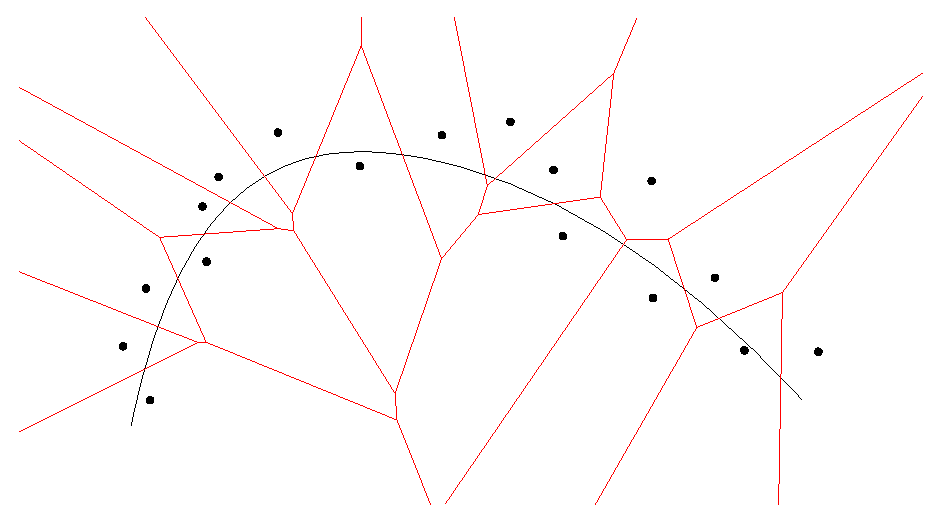
\includegraphics[scale=0.28]{img/voronoi-curve-2d}
        \hfill
        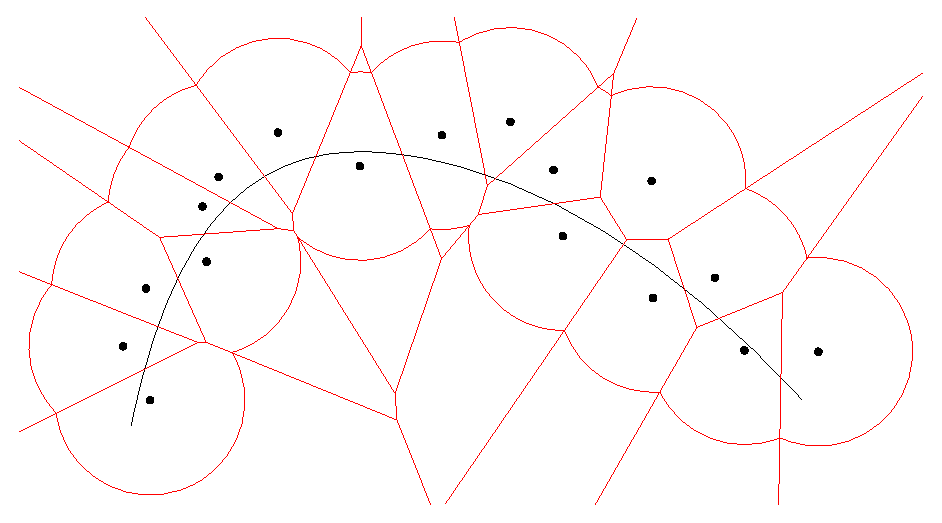
\includegraphics[scale=0.28]{img/voronoi-offset-2d}
    \end{figure}

    Then:
    \begin{align*}
        E(P^r) = E \left( \bigcup_p B(p, r) \right) &= \sum_p E(V(p, P) \cap P^r) \\
        &= \sum_p E(V(p, P) \cap B(p, r)) \\
    \end{align*}
\end{frame}

\subsection{Mean curvature estimation}
\begin{frame}
    \frametitle{Mean curvature estimation}
    % \framesubtitle{Examples}

    Examples: curvature of an ellipse
    \begin{figure}
        \centering
        \includegraphics[scale=0.3]{img/curvature-ellipse-200-15-area}
        \includegraphics[scale=0.3]{img/curvature-ellipse-200-15-perimeter}
        \caption{E = Area / E = Perimeter of the boundary}
    \end{figure}
\end{frame}

\subsection{Mean curvature flow}
\begin{frame}
    \frametitle{Mean curvature flow}
    % \framesubtitle{Examples}

    Examples: flow of a noisy ellipse
    \begin{figure}
        \centering
        \includegraphics[scale=0.22]{img/ellipse-200-noised-var-1-area}
        \includegraphics[scale=0.22]{img/ellipse-noised-area-5-01}

        \includegraphics[scale=0.22]{img/ellipse-200-noised-var-1-perimeter}
        \includegraphics[scale=0.22]{img/ellipse-noised-perimeter-7-2}
        \caption{Area / Perimeter of the boundary}
    \end{figure}
\end{frame}

\begin{frame}
    \frametitle{Mean curvature flow}
    % \framesubtitle{Examples}

    Results:
    \begin{itemize}
        \item Area and perimeter of the boundary: smoothing
        \item Area: creation of holes $ \to $ use weighted area
    \end{itemize}

    \begin{figure}
        \centering
        \includegraphics[scale=0.22]{img/ellipse-outliers}
        \includegraphics[scale=0.22]{img/ellipse-outliers-area}
        \includegraphics[scale=0.22]{img/ellipse-outliers-perimeter}
        \caption{Point cloud with outliers / area / perimeter of the boundary}
    \end{figure}
\end{frame}

\begin{frame}
    \frametitle{Properties}
    % \framesubtitle{Examples}

    Smoothing:
    \begin{figure}
        \centering
        \includegraphics[scale=0.2]{img/square}
        \includegraphics[scale=0.2]{img/square-smooth-area}
        \includegraphics[scale=0.2]{img/square-smooth-perimeter}
        \caption{Smoothing of the corners of a square}
    \end{figure}

    Area / perimeter minimization:
    \begin{figure}
        \centering
        \includegraphics[scale=0.2]{img/values-square-area}
        \includegraphics[scale=0.2]{img/values-ellipse-perimeter}
        \caption{Evolution of the area on a square / perimeter on an ellipse}
    \end{figure}
\end{frame}

% {{{1 3D
\section{3D case}

\subsection{Problem}
\begin{frame}
    \frametitle{Problem}
    % \framesubtitle{Anisotropic flow}

    Anisotropic flow:
    \begin{itemize}
        \item Union of balls $ \iff $ Union of convex polyhedra
        \item Choice of the polyhedron $ \to $ smoothing will be more important
            in some directions
    \end{itemize}

    Different methods:
    \begin{itemize}
        \item Naive (approximation): intersection between a Voronoi cell and a
            convex polyhedron
        \item Inclusion-exclusion formulae (approximation)
        \item 3D arrangements (exact?)
    \end{itemize}
\end{frame}

\begin{frame}
    \frametitle{Examples}
    % \framesubtitle{Polyhedra}

    Polyhedra:
    \begin{itemize}
        \item Discretization of a sphere: normal, mean curvature estimation
        \item Cube ($ L_{\infty} $ norm)
        \item Bipyramid ($ L_1 $ norm)
        \item Icosahedron
    \end{itemize}

    \begin{figure}
        \centering
        \includegraphics[scale=0.2]{img/sphere-polyhedron-200}
        \includegraphics[scale=0.2]{img/cube}
        \includegraphics[scale=0.2]{img/icosahedron}
    \end{figure}
\end{frame}

\begin{frame}
    \frametitle{Naive method}
    % \framesubtitle{Naive method}

    Idea: replace $ Vol(\bigcup_p B_N(p, r) \cap V(p, P)) $ by $ Vol(B_N(p, r) \cap V(p, P)) $

    \begin{figure}
        \centering
        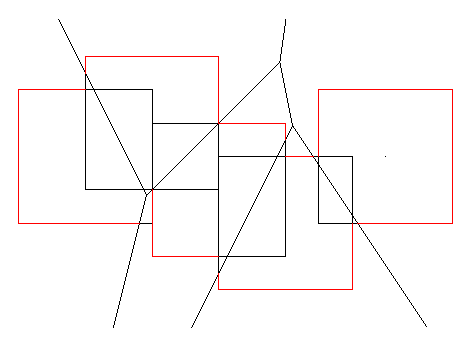
\includegraphics[scale=0.5]{img/3d_perimeter_squares}
        \hspace{2cm}
        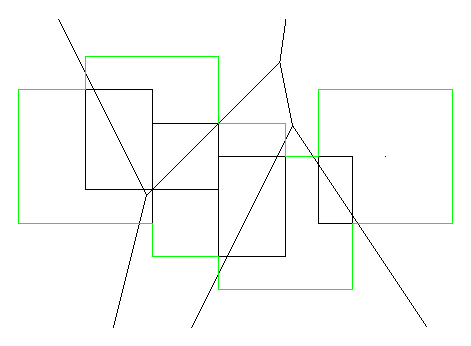
\includegraphics[scale=0.5]{img/3d_perimeter_squares_truth}
    \end{figure}

    \begin{figure}
        \centering
        \includegraphics[scale=0.2]{img/circle-cube-inter}
    \end{figure}
\end{frame}

\begin{frame}
    \frametitle{Inclusion-exclusion method}
    % \framesubtitle{Inclusion-exclusion method}

    Approximation of:

$$ \indicator{\bigcup B_N(p, r)} = \sum_{\sigma \in Nerve(\mathcal{B}_N)}
(-1)^{\dim \sigma} \indicator{\bigcap \sigma} $$

    where $ Nerve(\mathcal{B}_N) $ is replaced by $ Del(P, r) $: the
    $\alpha$-complex of $ P $ for $ \alpha = r $.

    Comparison of both methods:
    \begin{figure}
        \centering
        \includegraphics[scale=0.15]{img/cube-cube-15-naive}
        \includegraphics[scale=0.15]{img/cube-cube-15-ie}
    \end{figure}
\end{frame}

\subsection{Implementation}
\begin{frame}
    \frametitle{Implementation details}
    % \framesubtitle{Implementation details}

    Intersection computation:
    \begin{itemize}
        \item Voronoi cell and a convex polyhedron
        \item Half-space intersection
        \item Duality
    \end{itemize}

    Automatic differentiation integration:
    \begin{itemize}
        \item \emph{Kernel} parametrized by a number type
        \item Replace the number type by a custom class \texttt{AD}
        \item \texttt{AD} = value and a vector of derivatives + overloading and
            chain rule
    \end{itemize}

    Combination of two kernels:
    \begin{itemize}
        \item \texttt{Epick} for the exact combinatorics
        \item \texttt{Simple\_cartesian<AD>} for the construction
    \end{itemize}
\end{frame}

\subsection{Normal estimation}
\begin{frame}
    \frametitle{Normal estimation}
    % \framesubtitle{Examples}

    On a sphere:
    \begin{figure}
        \centering
        \includegraphics[scale=0.15]{img/sphere-1000}
        \includegraphics[scale=0.15]{img/sphere-sphere-1000-05}
    \end{figure}

    On the \texttt{fandisk} model:
    \begin{figure}
        \includegraphics[scale=0.18]{img/fandisk-normals}
    \end{figure}
\end{frame}

\subsection{Anisotropic flow}
\begin{frame}
    \frametitle{Anisotropic flow}
    % \framesubtitle{Examples}

    Cube: 10 iterations
    \begin{figure}
        \centering
        \includegraphics[scale=0.4]{img/sphere-cube-0}
        \includegraphics[scale=0.3]{img/sphere-cube-10}
        \includegraphics[scale=0.2]{img/sphere-cube-cube}
    \end{figure}

    Bipyramid: 10 iterations
    \begin{figure}
        \centering
        \includegraphics[scale=0.4]{img/sphere-cube-0}
        \includegraphics[scale=0.2]{img/sphere-bipyramid-10}
        \includegraphics[scale=0.2]{img/sphere-bipyramid-bipyramid}
    \end{figure}
\end{frame}

% {{{1 THEORY
\section{Theory}

\begin{frame}
    \frametitle{Theory}
    % \framesubtitle{Some results}

    Approximation of the area of a surface:
    \begin{block}{Proposition}
        Given an hypersurface $ S $, an $\epsilon$-sampling of $ S $: $ P $, we
        have:
        $$
            | \frac{Vol^d(P^r)}{2r} - A(S) | \leq \frac{\epsilon^2}{2r^2} +
            O \left(\frac{\epsilon^4}{r^3} \right) + O(r^2)
        $$
    \end{block}

    Convergence of the discretized gradient:
    \begin{block}{Proposition}
        Given an $\epsilon$-sampling $ P $ of a smooth ($ C^{\infty} $) hypersurface
        $ S $ and $ r \ge 0 $ such that: $ \epsilon \leq r \leq reach(M) $, then,
        for $ p = (p_1, \ldots, p_N) \in P^N $:
        $$
            \frac{\nabla_{p_i} A^r(p)}{r \times Vol^{d-1}(\partial B(p_i,r) \cap V(p_i,P))}
            = \meanv{S}(p_i) + O \left(\frac{\epsilon}{r}\right) + O(r)
        $$
    \end{block}
\end{frame}

% {{{1 PERSPECTIVES
\section{Perspectives}

\begin{frame}
    \frametitle{Perspectives}
    % \framesubtitle{Perspectives}

    \begin{itemize}
        \item Prove the convergence of the area of the boundary towards the mean
            curvature vector
        \item Better understanding of the gradient of the anisotropic flow:
            weight the area by the support function
        \item Improve the computation in 3D (use 3D arrangements?)
        \item Crystal growth simulation (anisotropic case)
    \end{itemize}
\end{frame}

\begin{frame}
    \frametitle{Perspectives}
    % \framesubtitle{PhD Thesis}

    PhD Thesis:
    \begin{itemize}
        \item Minimal surfaces: surface that minimizes its area while having a
            fixed boundary
        \item Anisotropic minimal surfaces
    \end{itemize}
\end{frame}

% \plain{Merci!}
\begin{frame}
    \begin{center}
        \huge{Thank you!}
    \end{center}
\end{frame}

\end{document}

% vim: set spelllang=en :
